\section{Kontinuerlig simulering}
\thispagestyle{fancy}

Parallelt med programmeringa har vi utført kontinuerlege testar og simuleringar av blokkene vi har utvikla. 
Dette har vært ein viktig del av vår arbeidsmetode. 

Kontinuerleg simulering er små testar som blir utført medan ein programmerar.
Det er ikkje ein isolert testfase med klare start- og stoppunkt, men heller små testar som gir ein indikasjon
på om arbeidet følgjer krav.

I denne oppgåva nytta vi kontinuerleg simulering i programmering av alle blokker.
\gls{IEC} blokkene hadde mange funksjonar som ikkje var avhengige av kvarandre,
som gjorde det mogleg å gjennomføre små, enkle testar utan at heile blokka var ferdigstilt.\newline
Som eit døme, skal RX resete ein utgang Y. Dette blir implementert og deretter testa ved hjelp av simulering.
Kva som til slutt skal sette utgangen Y høg er ikkje relevant i dette tilfellet. Vi har implementert 
og testa at ein reset vil fungere.


\begin{figure}[htbp]
    \centering
    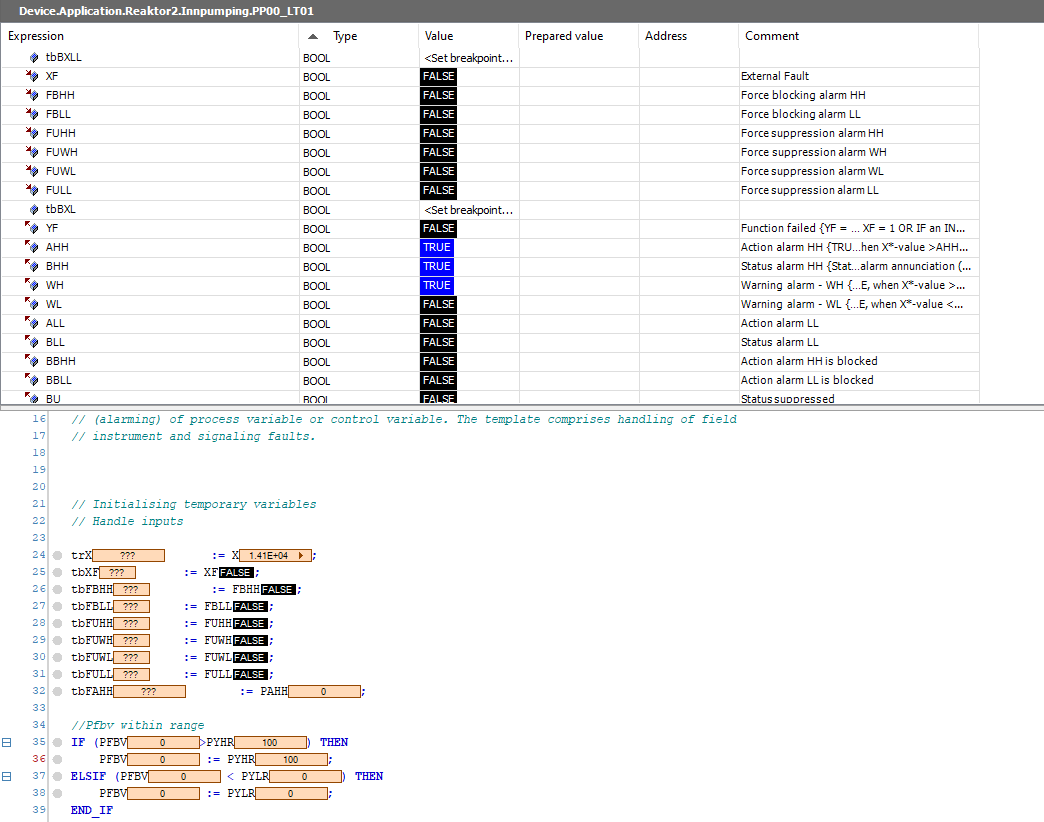
\includegraphics[width=0.8\textwidth]{Bilder/kontinuerligSimulering.png}
    \caption{Kontinuerleg testing ved manipulasjon av verdiar}\label{fig:KontinuerlegSimulering}
\end{figure}


\newpage
